\paragraph{phase 1}
We input "1+1=", "!", "2\&", "3/0=", "4+4~" successively to the serial monitor after we run the project. The output result of the serial monitor is shown in figure[\ref{fig:test1}]. The output result on LCD is the same as expected.
\begin{figure}[!htbp]
	\centering
	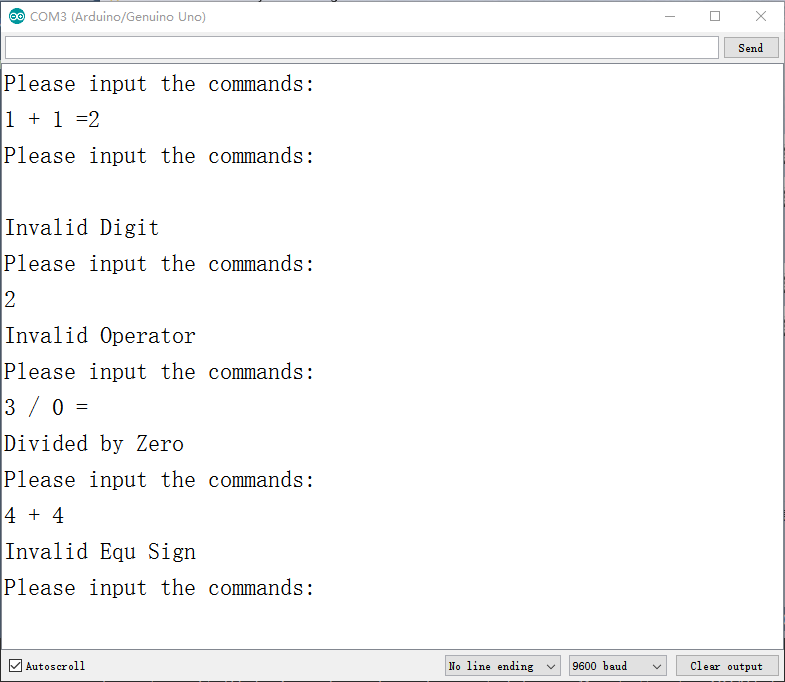
\includegraphics[width = \linewidth]{images/test1.png}
	\caption{Test result on serial monitor for phase 1}
	\label{fig:test1}
\end{figure}

\paragraph{phase 2}
We input "12+24=", "35*3", "34+!", "79\&", "67+90-", "87/00=" successively to the serial monitor after we run the project. The output result of the serial monitor is shown in figure[\ref{fig:test2}]. The output result on LCD is the same as expected.
\begin{figure}[!htbp]
	\centering
	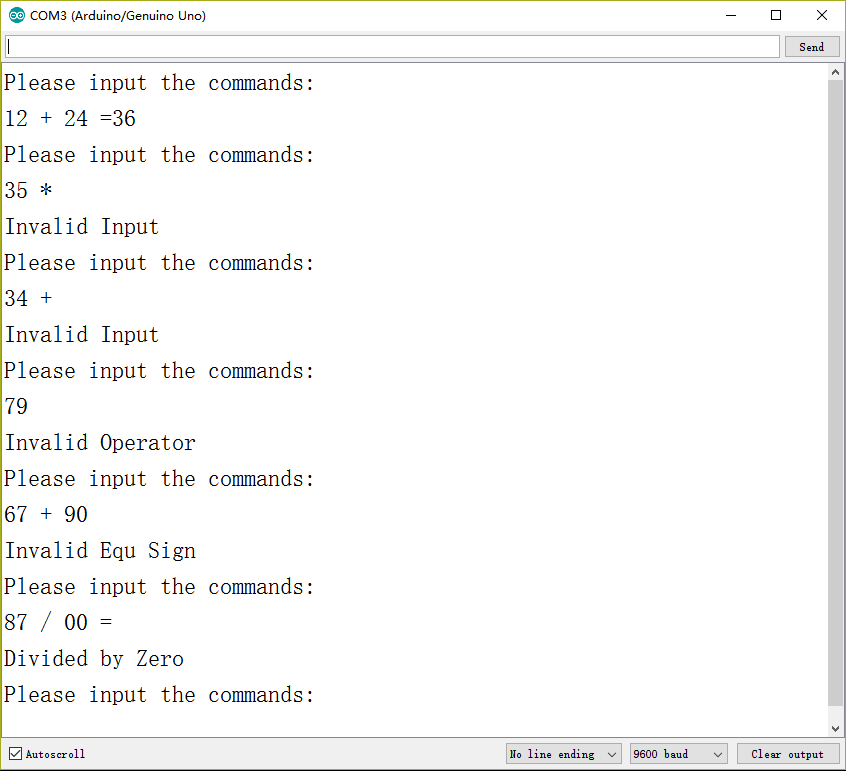
\includegraphics[width = \linewidth]{images/test2.png}
	\caption{Test result on serial monitor for phase 2}
	\label{fig:test2}
\end{figure}

\paragraph{phase 3}
We input "39-67=", "48(", "~", "28*45+", "90/00=", "-89*-23=", "78/-46=" successively to the serial monitor after we run the project. The output result of the serial monitor is shown in figure[\ref{fig:test3}]. The output result on LCD is the same as expected.
\begin{figure}[!htbp]
	\centering
	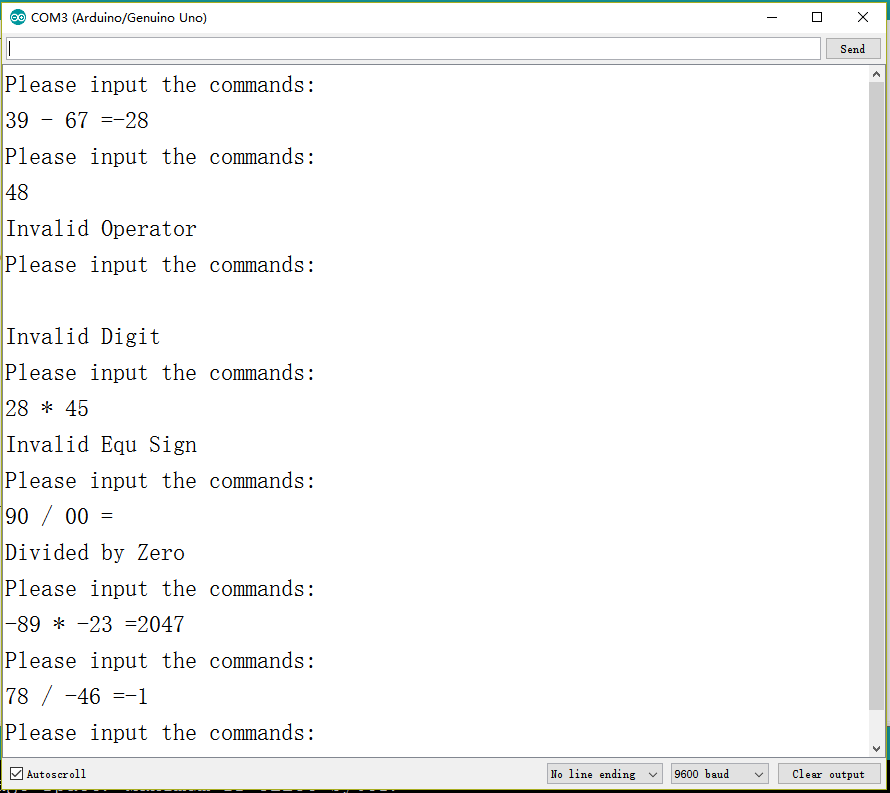
\includegraphics[width = \linewidth]{images/test3.png}
	\caption{Test result on serial monitor for phase 3}
	\label{fig:test3}
\end{figure}

\paragraph{two processors}
We input "12+29=", "42(", "3", "29*35+", "34/00=", "67+-38=" successively to the serial monitor of the master processor after we run the project on both processors. The output result of the serial monitor of the master and slave processors is shown in figure[\ref{fig:test4}]. The output result on LCD of the slave processor is the same as expected.
\begin{figure}[!htbp]
	\centering
	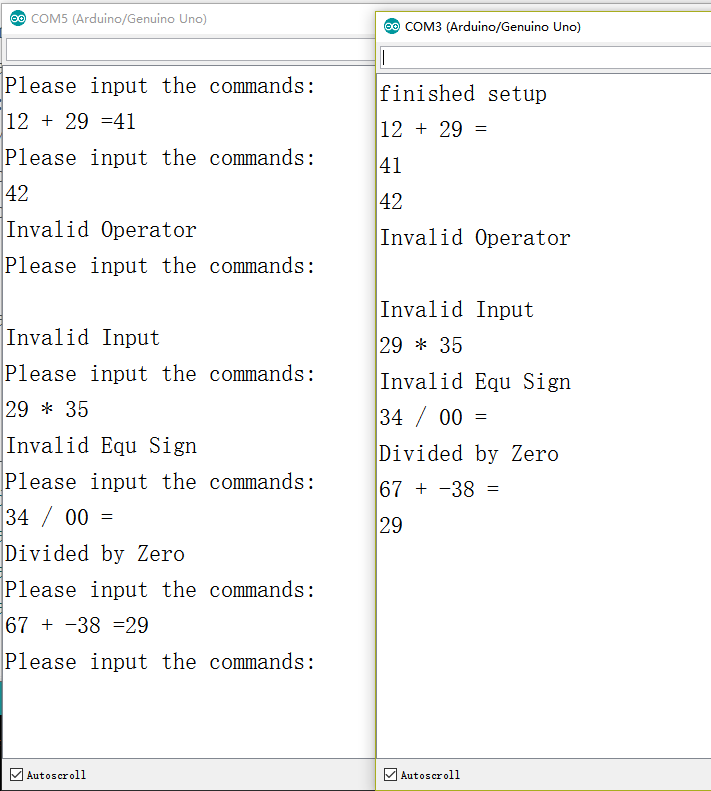
\includegraphics[width = \linewidth]{images/test4.png}
	\caption{Test result on serial monitor for phase 4}
	\label{fig:test4}
\end{figure}
